\documentclass{emulateapj}
\bibliographystyle{apj}

%define general packages
\usepackage{epsfig}
\usepackage{rotating}
\usepackage{amsmath}
\usepackage{footnote}
\usepackage{setspace}
\usepackage{courier}


\begin{document}

\title{A Fiber Collision Correction Method for the BOSS Power Spectrum} 

\author{ChangHoon~Hahn\altaffilmark{1}, 
Roman~Scoccimarro\altaffilmark{1}, 
Michael R.~Blanton\altaffilmark{1}, others} 
\altaffiltext{1}{Center for Cosmology and Particle Physics, Department of Physics, New York University, 4 Washington Place, New York, NY 10003; chh327@nyu.edu}

\begin{abstract}
Fiber-fed multi-object spectroscopic surveys, with their ability to collect an unprecedented number of redshifts, dominate cosmological studies. However physical constraints limit these surveys from successfully collecting redshifts from galaxies that are too close to each other on the focal plane, which ultimately leads to significant systematic effects on galaxy clustering measurements. Using simulated mock catalogs, extensively used in interpreting large-scale structure clustering results of the Sloan Digital Sky Survey, we investigate the effects of fiber collisions on the galaxy power spectrum and compare the methods currently used to correct for fiber collisions in the literature and assess their success in reconstructing the true power spectrum. 

We present our fiber collision correction method, which first statistically reconstructs the clustering of fiber collided pairs by modeling the distribution of the line-of-sight displacements between them using cases where both redshifts are obtained. The method properly accounts for fiber collisions in the shot-noise correction term of the power spectrum estimator. Using our method, we successfully reproduce the true power spectrum for the mock catalogs with residuals of $< 1\%$ at $k \sim 0.3 \; h/\mathrm{Mpc}$ and $< 10\%$ at $k \sim 0.8 \; h/\mathrm{Mpc}$. Our comparisons to other existing correction methods demonstrate that our method most accurately reconstructs the true power spectrum from fiber collided galaxy data especially at small scales ($k > 0.1\; h/\mathrm{Mpc}$), with the added advantage that our method can be validated and calibrated in observed data. With statistical uncertainty no longer dominating galaxy clustering measurements, our correction method will allow us to extend power spectrum measurements to smaller scales than previously possible. 
\end{abstract}
\keywords{cosmology: observations -- cosmology: large-scale structure of universe -- galaxies: distances and redshift -- galaxies: halos -- galaxies: statistics}

\section{Introduction} 
As of 2015, millions of redshifts to distant galaxies have been obtained through redshift surveys. Cosmological measurements such as galaxy clustering statistics are no longer dominated by uncertainties from statistical precision, but from systematic effects of the measurements. These surveys, such as the 2dF Galaxy Redshift Survey (2dFGRS; \citealt{Colless:1999aa}) and the Sloan Digital Sky Survey III Baryon Oscillation Spectroscopic Survey (SDSS-III BOSS; \citealt{Anderson:2012aa, Dawson:2013aa}) and future surveys such as the Extended Baryon Oscillation Spectroscopic Survey (eBOSS; {\bf WHO DO CITE?}) use fiber-fed spectrographs. 

For each galaxy, a fiber is used to obtain a spectroscopic redshift. However, due to the physical size of the fiber housing, if two galaxies are located within the fiber collision angular scale from one another on the sky, separate fibers cannot be placed adjacently to observe them simultaneously (\citealt{Yoon:2008aa} {\bf CITE MORE}). In these situations, only a single redshift is measured. With redshifts of galaxies in close angular proximities missing from the sample, any clustering statistic probing these scales will be systematically affected. 

As our cosmological surveys extend further to higher redshifts, the systematic effect becomes more severe because the fiber collision angular scale corresponds to a larger comoving scale, thereby affecting our measurements on larger scales. SDSS-III BOSS, in particular, has an angular fiber collision scale of $62''$. This corresponds to $\sim 0.4 \;\mathrm{Mpc}/h$ at the center of the survey's redshift redshift range; fiber collided galaxies account for $\sim 5\%$ of the galaxy sample (\citealt{Anderson:2012aa}). Although this accounts for a relatively small fraction of redshifts, its effect on clustering measurements such as the power spectrum is significant. They must to be accounted for to probe smaller scales and higher order statistics such as the three-point correlation function or the bispectrum. Even with the use of robotic fiber positioner technology in future surveys such as the Dark Energy Survey Instrument (DESI; \citealt{Schlegel:2011aa, Morales:2012aa, Makarem:2014aa}) 
% What is the fiber positioner areas called??
will render fiber collisions obsolete. Therefore, accounting for the systematic effects remains an unavoidable challenge for clustering statistics. 

To correct for fiber collisions, one common approach used in clustering statistics is the nearest neighbor method (\citealt{Zehavi:2002aa, Berlind:2006aa, Anderson:2012aa}). For fiber collided galaxies without resolved redshifts, the method assigns the statistical weight of the fiber collided galaxy to its nearest angular neighbor. This provides a reasonable correction for the fiber collision effects at scales much larger than the fiber collision scales; however the correction falls short near the fiber collision scale. In fact, as \cite{Zehavi:2005aa} find, fiber collisions affect the two-point correlation function (2PCF) measurements even on scales significantly larger than the fiber collision scale ( $> 1\;\mathrm{Mpc}/h$). For power spectrum measurements in BOSS, the nearest neighbor method has often been supplemented with adjustments in the constant shot-noise term of the power spectrum estimator to correct for fiber collisions (\citealt{Beutler:2014aa, Gil-Marin:2014aa}). While this shot-noise term adjustment has been calibrated within the mock catalogs used to interpret the BOSS clustering results there is no way to validate and calibrate these methods independently for observations. Methods of this kind rely entirely on the accuracy of the mock catalogs to constrain fiber collisions, which is especially concerning since fiber collisions systematically affect small scales and mock catalogs may not be realiable at such small scales (\citealt{Heitmann:2008aa, Schneider:2015aa}). 

Recently \cite{Guo:2012aa}, focusing on SDSS-III BOSS like samples, proposed a fiber collision correction method for the 2PCF that is able to reasonably correct for fiber collisions above and below the collision scale. \cite{Guo:2012aa} estimates the total contribution of fiber collided galaxies to the two point correlation function by examining the pair statistics in overlapping tiling regions of the survey, where a smaller fraction of galaxies suffer from fiber collisions. Unfortunately, due to the complex geometry of the overlapping regions, this method is difficult to apply to Fourier clustering measurements. As a result, we propose a fiber collision correction method that, first, improves upon the nearest neighbor method by using the distribution of the line-of-sight displacement between resolved fiber collided galaxies to statistically reconstruct the clustering of fiber collided galaxies; and properly accounts for fiber collisions in the shot-noise correction term of the power spectrum estimator. 

In Section \ref{sec:catalog}, we present a brief description of the simulated mock catalogs with realistically applied fiber collisions and the power spectrum estimator used throughout the paper. Then during our discussion of the two components of our correction method in Section \ref{sec:fc_corr}, we quantify the effects of fiber collisions of power spectrum measurements and test and compare correction methods in the literature. Afterwards, we present our correction method, test it on the mock catalogs, and compare it to other correction methods in Section \ref{sec:results}. Finally in Section \ref{sec:summary} we summarize and discuss our results. 

%%%%%%%%%%%%%%%%%%%%%%%%%%%%%%%%%%%%%%%%%%%%%%%%%%%%%%%%%%%%%%%%%%%%%%%%%%%%%%
% fiber collided Mock catalogs
%%%%%%%%%%%%%%%%%%%%%%%%%%%%%%%%%%%%%%%%%%%%%%%%%%%%%%%%%%%%%%%%%%%%%%%%%%%%%%
\section{fiber collided Mock catalogs} \label{sec:catalog}
For various purposes such as calculating covariance matrices or estimating cosmic variance, simulated mock catalogs play a crucial role in interpreting clustering measurements of observed galaxies (\citealt{Scoccimarro:2002aa, Anderson:2012aa, Manera:2013aa}). They also provide a means of understanding systematic effects such as fiber collisions (\citealt{Guo:2012aa, Manera:2013aa} {\bf LIST MORE}) since systematic effects can be simulated on the mock catalogs. This allows us to test how these effects influence clustering measurements and devise correction methods that attempt to account for these effects.

A direct way of understanding the effects of fiber collisions on clustering statistics in observations is to first apply fiber collisions to mock catalogs and then compare the clustering statistics obtained from mock catalogs with and without the fiber collisions. Correction methods for fiber collisions can then be applied to the fiber collided mocks and the merit of the correction method can be quantified by how successfully they reproduce the clustering statistics of the original mock catalogs without fiber collisions. The optimal correction method can then be applied to the observed data with some assurance that it accounts for fiber collisions and improves the clustering measurements. 

When applying the fiber collisions to the mock catalogs, it is essential to apply them in the same manner they affect the observational data. For BOSS, galaxies within $62"$ are fiber collided (\citealt{Anderson:2012aa}). In reality, this simple criteria is further complicated by the tiling scheme of observing plates that create overlapping regions, which have a higher success rate in resolving galaxy spectra within the fiber collision angular scale (\citealt{Guo:2012aa}). Furthermore, fiber collisions are only one of the systematic effects that influence BOSS data. Systematic effects include the unique geometry of the BOSS survey, the variable completeness in different sectors of the survey, and redshift failures (\citealt{Anderson:2012aa}). 

\def \cmasscolor{black}
\def \ldgcolor{blue}
\def \qpmcolor{orange}
\def \tmcolor{green}
\begin{figure}
\begin{center}
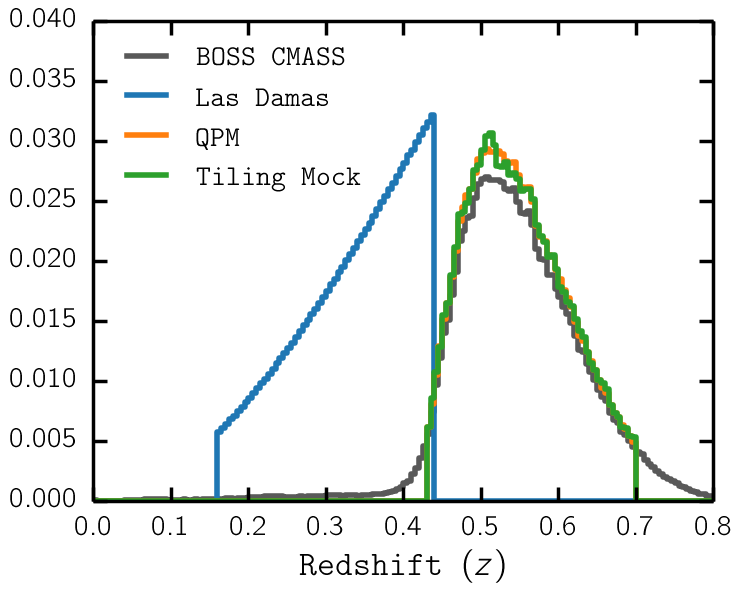
\includegraphics[scale=0.45]{fcpaper_z_dist.png} \label{fig:zdist}
\caption{Normalized galaxy redshift distribution for LasDamas (\ldgcolor), QPM (\qpmcolor), and Tiling Mock (\tmcolor) mock catalogs. The normalized redshift distribution of BOSS DR12 CMASS is also plotted (\cmasscolor). Bin size of $\Delta z = 0.025$ was used to compute the each of the distributions. LasDamas mock catalog has a constant number density of galaxies throughout $0.16 < z < 0.44$, the redshift range of SDSS LRG sample. QPM and Tiling Mock catalogs, on the other hand, trace the BOSS CMASS redshift distribution ($0.43 < z < 0.7$).}
% perhaps the range should be wider and make it full text width that way the tail can be portrayed better. Keep the same aspect ratio. 
\end{center}
\end{figure}

Effects of fiber collisions must be understood and interpreted in conjunction with these other systematic effects. Therefore, in this paper, we use LasDamas (\citealt{McBride:2009aa, McBride:2011aa}), Quick Particle Mesh (\citealt{White:2014aa}), and Tiling mock catalogs ({\bf CITATIONS?}), which have already been extensively used in interpreting clustering results for SDSS and BOSS and are generated through different prescriptions. Therefore they provide unique data sets to measure the effects of fiber collisions and to test our correction method tailored for BOSS. 
%Each of these mock catalogs use some sort of N-body dark matter simulation along with a HOD prescription to populate the dark matter halos with ``galaxies". % Include brief detail on what each mock has to offer

The LasDamas Galaxy mock catalogs are constructed from the Oriana N-body Large Suite of Dark Matter Simulations (LasDamas) with $1280^3$ particles with a box with side length, $L_\mathrm{Box} = 2400\;\mathrm{Mpc}/h$. The N-body LasDamas simulations use a spatially flat $\Lambda$CDM cosmology with $\Omega_\mathrm{m} = 0.25$, $\Omega_\Lambda = 0.75$, $\Omega_\mathrm{b} = 0.04$, $\sigma_8 = 0.8$, $n_\mathrm{s} = 1$ and $h=0.7$. The dark matter halos are then identified using a friends-of-friends (FOF) algorithm (\citealt{Davis:1985aa}) with a linking length $b = 0.2 $ times the mean interparticle separation. The over-densities of dark matter halos are then populated with galaxies using the halo occupation distribution (HOD) framework to construct the galaxy mock catalogs (\citealt{McBride:2009aa, McBride:2011aa}). The HOD prescription is specified so that the galaxy mock catalogs reproduce the galaxy number density and projected correlation function of the observed SDSS Luminous Red Galaxy sample with $M_g < -21.8$. The LasDamas galaxy mock catalogs have 40 realizations, each of which spans the redshift range, $0.16 < z < 0.44$ and are restricted to the survey geometry of SDSS Data Release 7. They also include redshift space distortions from velocities, but do not model fiber collisions. 

To model the fiber collisions of the observed galaxies in BOSS, we impose fiber collisions at the angular scale of $62''$. Once we identify galaxies within $62''$ of each other, we arbitrary select one of the galaxies and assign the statistical weights of the other galaxies within $62''$ of it. Roughly $\sim 2.5 \%$ of the galaxies in the LasDamas mock catalogs are affected by fiber collisions. 

Next, the QPM mock galaxy catalogs uses a ``quick particle mesh" method, which uses a low resolution particle-mesh N-body solver to evolve particles within a period simulation volume. The particles are assigned halo masses  in order to match the halo mass function and large-scale bias of halos of high resolution simulations. Afterward the \cite{Tinker:2012aa} HOD parameterization is used to populate the halos. The mock galaxy sample is then trimmed to the BOSS CMASS survey footprint, downsampled based on angular sky completeness (sector completeness) and radial selection. Furthermore, QPM mocks model the fiber collisions of the BOSS CMASS sample ($62''$ angular fiber collision scale). The QPM galaxy mock catalog uses the following $\Lambda$CDM cosmology: $\Omega_\mathrm{m} = 0.29$, $\Omega_\Lambda = 0.71$, $\sigma_8 = 0.8$, $n_\mathrm{s} = 0.97$ and $h=0.7$. We use 1000 realizations of the QPM galaxy mock catalog. For a detailed description of the QPM galaxy mock catalogs we refer readers to \cite{White:2014aa}. 

Finally the Tiling Mock catalog is generated using 

{\bf INSERT TILING MOCK DESCRIPTION HERE}

In Figure \ref{fig:zdist}, we plot the redshift distribution for LasDamas, QPM, and Tiling Mock catalogs along with the redshift distribution of BOSS DR12 galaxies. The LasDamas mock catalog, which is constructed based on the SDSS LRG sample has a constant $\bar{n}(z)$ over the redshift $0.16 < z< 0.44$, while the QPM and Tiling mock redshift distributions closely trace the observed BOSS redshift distribution (roughly $0.43 < z < 0.7$). 

\subsection{Power Spectrum Estimator} \label{sec:pk_est}
In this paper, we focus on the effects of fiber collisions on the galaxy power spectrum out of the other clustering measurements. Throughout the paper, when we measure the power spectrum, we use the standard \cite{Feldman:1994aa} (hereafter FKP) estimator and the following formalisms from the FKP paper: 
\begin{equation} \label{eq:fkppk}
P({\bf k}) = <|F({\bf k})|^2> - \frac{(1+\alpha) \int d^3r \;\bar{n}({\bf r})w_{\mathrm{FKP}}^2({\bf r})} {\int d^3r \; \bar{n}^2({\bf r})w_{\mathrm{FKP}}^2({\bf r})},
\end{equation}  
where
\begin{equation}
F({\bf r}) = \frac{w_\mathrm{FKP}({\bf r}) [n_g({\bf r}) - \alpha n_r({\bf r})]} {[\int d^3r \; \bar{n}^2({\bf r})w_\mathrm{FKP}^2({\bf r})]^{\frac{1}{2}}} 
\end{equation}
and the second term represents the constant shot-noise contribution to the power due to the discrete density field of our galaxies. $n_g$ is the galaxy density, $n_r$ is the density of the synthetic random catalog, $\alpha$ is the ratio of the number of galaxies over the number of synthetic random galaxies, $\bar{n}$ is the mean density of the galaxies, and $w_{\mathrm{FKP}}$ is the minimum variance weight derived in \cite{Feldman:1994aa}: 
\begin{equation}
w_{\mathrm{FKP}} ({\bf r}) = \frac{1}{1+\bar{n}({\bf r}) P_0}
\end{equation}
where $P_0$ is the power spectrum amplitude at which the error is minimized. We use $P_0 = 20000\; \mathrm{Mpc}^3/h^3$ for our analysis, which corresponds to $k \sim 0.1\; h/\mathrm{Mpc}$.  

\begin{figure}
\begin{center}
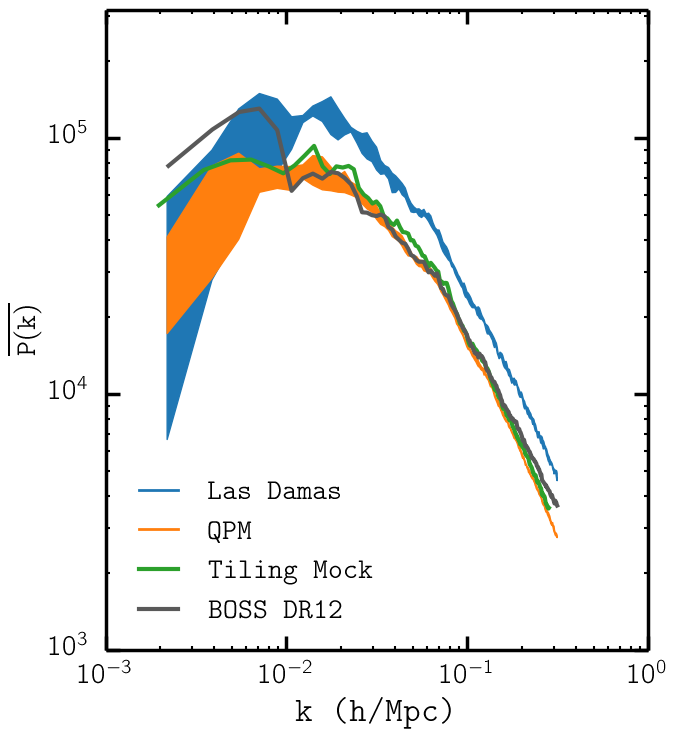
\includegraphics[scale=0.5]{fcpaper_pk_comp.png} 
\caption{Average power spectrum $\overline{P(k)}$ for BOSS DR12 (black) and the mock catalogs LasDamas (blue), QPM (orange), and Tiling Mock (green), listed in Section \ref{sec:catalog} using the FKP $P(k)$ estimator. The width of the $P(k)$ for LasDamas and QPM represent the sample variance ($\Delta P(k)$) calculated from the multiple realizations of the mock catalogs. We emphasize that fiber collisions were not applied to the mock catalogs for the $P(k)$ measurements. Meanwhile, galaxy weights (Equation \ref{eq:weight}) are applied to the BOSS DR12 $P(k)$ measurement. We remind readers that the LasDamas mock catalog has an overall greater $\overline{P(k)}$ due to the fact that the catalog spans the SDSS LRG sample redshift range instead of the BOSS redshift range of the other mock catalogs.} \label{fig:mockpk}
\end{center}
\end{figure}

For LasDamas, QPM, and Tiling mock catalogs we use the FKP estimator described above to measure the power spectrum in Figure \ref{fig:mockpk}. The fiber collisions described previously are not applied to the mock catalogs in the $P(k)$ calculations for Figure \ref{fig:mockpk}. Without fiber collisions, we use the exact formulation of Equation \ref{eq:fkppk} in the FKP power spectrum estimator. 

We also plot the $P(k)$ from the BOSS Data Release 12 CMASS data (\cmasscolor) in Figure \ref{fig:mockpk}. For BOSS DR12 CMASS, systematic weights are assigned to the galaxies in order to account for sector completeness, redshift failures, and fiber collisions. Each galaxy has a statistical weight determined by, 
\begin{equation} \label{eq:weight}
w_\mathrm{tot} = w_\mathrm{sys} (w_\mathrm{rf} + w_\mathrm{fc} -1), 
\end{equation} 
(\citealt{Anderson:2012aa, Beutler:2014aa}). As a result, we modify Equation \ref{eq:fkppk} when we calculate the power spectrum. Instead of the galaxy density term $n_g({\bf r})$ we use a weighted galaxy density term $n'_g({\bf r}) = n_g({\bf r}) w({\bf r})$, which includes the systematic weights for each galaxy. Also, instead of $\alpha = N_{\mathrm{gal}}/N_\mathrm{ran}$ we use $\alpha ' = N'_\mathrm{gal}/N_\mathrm{ran}$ where $N'_\mathrm{gal} = \sum_\mathrm{gal} w_\mathrm{tot}$. 

For LasDamas and QPM, which have multiple realizations, we compute the sample variance of the power spectrum
\begin{equation} \label{eq:pk_var}
\Delta P (k)= \sqrt{\frac{1}{N_\mathrm{realization}} \sum\limits_i^{N_\mathrm{realization}} (P_i(k)- \overline{P(k)})^2 }. 
\end{equation}
$N_\mathrm{realization}$ is the total number of realizations (40 for LasDamas and 1000 for QPM) and $P_i(k)$ is the power spectrum for each realization. $\Delta P(k)$ is represented by the width of the $P(k)$ in Figure \ref{fig:mockpk}. 

\begin{figure*}
\begin{center}
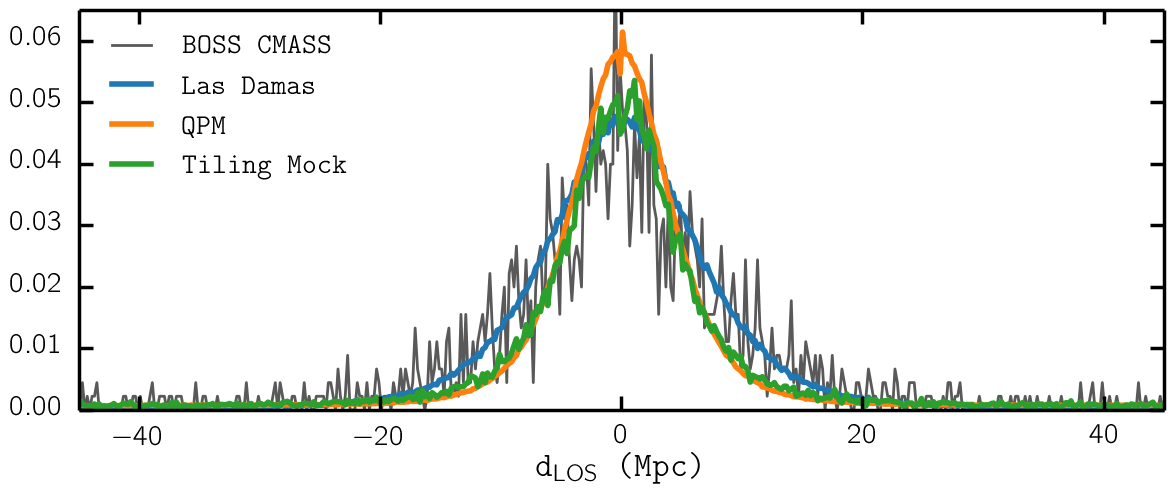
\includegraphics[scale=0.575]{fcpaper_dlos_dist.png}
\caption{Normalized distribution of $d_{\mathrm{LOS}}$ for LasDamas (\ldgcolor), QPM (\qpmcolor), and Tiling Mock (\tmcolor) mock catalogs. The normalized $d_{\mathrm{LOS}}$ distribution of BOSS DR12 is also plotted (\cmasscolor). Bin size of $\Delta d = 0.2$ was used to compute the $d_{\mathrm{LOS}}$ distributions. The $d_\mathrm{LOS}$ distribution extends to $\sim \pm 500 \; \mathrm{Mpc}$ (not shown above). We focus on the peak of the distribution $-20 \; \mathrm{Mpc} < d_\mathrm{LOS} < 20 \;\mathrm{Mpc}$ (discussed in \ref{sec:dlos}).} \label{fig:d_los}
% perhaps the range should be wider and make it full text width that way the tail can be portrayed better. Keep the same aspect ratio. 
\end{center}
\end{figure*}

%%%%%%%%%%%%%%%%%%%%%%%%%%%%%%%%%%%%%%%%%%%%%%%%%%%%%%%%%%%%%%%%%%%%%%%%%%%%%%
% fiber collision Correction Method
%%%%%%%%%%%%%%%%%%%%%%%%%%%%%%%%%%%%%%%%%%%%%%%%%%%%%%%%%%%%%%%%%%%%%%%%%%%%%%
\section{fiber collision Correction Method} \label{sec:fc_corr}
As mentioned above, a common approach in accounting for fiber collisions in clustering measurements has been to use the nearest angular neighbor method (\citealt{Zehavi:2002aa, Berlind:2006aa, Anderson:2012aa}). For galaxies without resolved spectroscopic redshifts due to fiber collisions, the entire statistical weight of the galaxy is assigned to its nearest angular neighbor. This method effectively assumes that all galaxies within the angular fiber collision scale ($< 62 "$ for BOSS) are correlated with one another. In other words, the method assumes that galaxies within the fiber collision angular scale reside in the same halo so displacing one and placing it on top of the other does not significantly alter the clustering statistics. One consequence of this method however is that galaxies within the angular fiber collision scale purely by coincidence (hereafter referred to as ``chance alignments") are incorrectly assumed to be gravitationally correlated, so when their statistical weight is added to its nearest angular neighbor, they are in fact displaced significantly from their true position. For BOSS, the nearest angular neighbor method can displace galaxies by up to $500 \;\mathrm{Mpc}$. Furthermore even for fiber collided galaxies that reside in the same group or cluster, up-weighting the nearest neighbor ignores halo-scale line-of-sight displacements, which as we present in Section \ref{sec:dlos}, are significant. 

Although the nearest-neighbor method provides a reasonable estimate at large scales, in Section \ref{sec:dlos} we demonstrate that at small scales its effects on the power spectrum are significant and dominate sample variance. We present an improved method to account for correlated fiber collided galaxies using the line-of-sight displacement between fiber collided pairs. Then in Section \ref{sec:shotnoise}, we present modifications to the FKP power spectrum estimator in order to properly account for fiber collisions through the shot-noise correction term in the estimator. 

% MAKE SURE IT IS CLEAR THAT OUR CORRECTION METHOD COMBINES THE TWO. 


%%%%%%%%%%%%%%%%%%%%%%%%%%%%%%%%%%%%%%%%%%%%%%%%%%%%%%%%%%%%%%%%%%%%%%%%%%%%%%
% LOS DISPLACEMENT
%%%%%%%%%%%%%%%%%%%%%%%%%%%%%%%%%%%%%%%%%%%%%%%%%%%%%%%%%%%%%%%%%%%%%%%%%%%%%%
\subsection{Line-of-Sight Displacement of fiber collided Pairs} \label{sec:dlos}
It is impossible to determine definitely from observed galaxy data whether individual fiber collided galaxies without resolved spectroscopic redshift are correlated or chance alignments. Fortunately, using the fiber collided pairs with resolved redshifts (mainly in the overlapping regions mentioned in Section \ref{sec:catalog}), it is possible to model the line-of-sight displacement of the fiber collided pairs and the fraction of galaxy pairs that are corrected and uncorrelated. 

For simulated mock catalogs, described in Section \ref{sec:catalog}, modeling the fiber collided galaxy pairs is a much more direct task since fiber collisions are post-processed after the simulated galaxy positions are generated. All redshift values are provided for all galaxies regardless of angular proximity and the fiber collisions imposed on the mock catalogs are represented through the galaxies' ``fiber collision weights" ($w_\mathrm{fc}$). So for a fiber collided pair, one galaxy (``the nearest neighbor") will have the fiber collision weight of both galaxies, while the other has $w_\mathrm{fc} = 0$. Nonetheless, with redshifts of both fiber collided pair galaxies in mock catalogs, we can model the correlated and uncorrelated fiber collided pairs in order to better correct for fiber collisions. 

To determine whether or not fiber collided pairs are correlated, we examine the comoving line-of-sight displacement ($d_{\mathrm{LOS}}$) of fiber collided galaxy pairs. We calculate the $d_{\mathrm{LOS}}$ by taking the difference of the line-of-sight comoving distance from the resolved redshifts: 
\begin{equation}
d_{\mathrm{LOS}} = D_{\mathrm{C}} (z_1) - D_{\mathrm{C}} (z_2). 
\end{equation}
$D_{\mathrm{C}}(z)$ is the line-of-sight comoving distance at redshift $z$ (\citealt{Hogg:1999aa}). $z_1$ and $z_2$ represent the resolved redshifts of the galaxies in the fiber collided pair.

After calculating the $d_{\mathrm{LOS}}$ for every fiber collided pairs, in Figure \ref{fig:d_los} we present the distribution of $d_{\mathrm{LOS}}$ for LasDamas (\ldgcolor), QPM (\qpmcolor), Tiling Mock (\tmcolor), and BOSS DR12 (\cmasscolor). All of the $d_{\mathrm{LOS}}$ distributions contain two components: a peak contained within the range $-20\;\mathrm{Mpc} < d_{\mathrm{LOS}} < 20\;\mathrm{Mpc}$ and a flat component (hereafter "tail" component) outside the peak that extends to $d_{\mathrm{LOS}} \sim \pm 500 \;\mathrm{Mpc}$ (entire range of the distribution not displayed in Figure \ref{fig:d_los}). For the BOSS data, since we cannot compute the $d_\mathrm{LOS}$ for fiber collided pairs without spectra, the $d_\mathrm{LOS}$ distribution only reflects the $d_\mathrm{LOS}$ from fiber collided pairs {\em with} resolved spectroscopic redshifts, mostly from tile overlapping regions of the BOSS survey.

Galaxies within the same halo, due to their gravitational interactions at halo-scales, are more likely to be in close angular proximity with each other. These galaxies in over-dense regions cause the peak in the $d_{\mathrm{LOS}}$ distribution. The ``tail" component is composed of chance alignment galaxy pairs that happen to be in close angular proximity. 

Focusing on the peak of the distribution, we note that it closely traces an Gaussian function. Therefore, we fit a Gaussian of the form, 
\begin{equation} \label{eq:peak} 
p(d_{\mathrm{LOS}}) = A \; e^{-{d_{\mathrm{LOS}}^2}/{2\sigma^2}}
\end{equation}
 for a mathematical prescription of the $d_{\mathrm{LOS}}$ distribution peak as a function of the displacement for each of the data catalogs in Figure \ref{fig:d_los}. The best-fit $\sigma$ and $A$ parameters are obtained by fitting Equation \ref{eq:peak} to the $d_{\mathrm{LOS}}$ distribution peaks using MPFIT (\citealt{Markwardt:2009aa}). We list the values of $\sigma$ obtained for the mock catalogs in Table \ref{tab:mpfit}. Both Table \ref{tab:mpfit} and Figure \ref{fig:d_los} illustrate that the $d_{\mathrm{LOS}}$ distributions for the mock catalogs closely trace the distribution of the BOSS DR12, which further goes to support the use of mock catalogs in our investigation of fiber collisions.  
 
 \begin{table} 
 \caption{$d_{\mathrm{LOS}}$ Distribution Best-fit Parameters} \label{tab:mpfit}
 \begin{spacing}{1.5}
 \begin{center}
 \leavevmode
 \begin{tabular}{ccc} \hline \hline
catalog &$\sigma$ ($\mathrm{Mpc}$) & $f_{\mathrm{peak}}$\\ \hline
LasDamas 	& 6.85	& 0.71 \\ 
QPM 		& 4.98	& 0.65 \\ 
Tiling Mock 	& 5.38	& 0.57 \\ 
BOSS DR12 	& 7.6		& 0.65 \\ \hline
\end{tabular} \par
\end{center}
\end{spacing}
%    \bigskip 
{\bf Notes}: Best-fit parameter $\sigma$ and peak fraction $f_{\mathrm{peak}}$ for the $d_{\mathrm{LOS}}$ distributions in Figure \ref{fig:d_los}. 
\end{table}

Using the best-fit to the peak of the $d_{\mathrm{LOS}}$ distribution, we estimate the fraction of fiber collided pairs that are within the peak: 
\begin{equation}
f_{\mathrm{peak}} = \frac{\sum\limits_{\mathrm{peak}} p(d_{\mathrm{LOS}})}{N_{\mathrm{pairs}}}, 
\end{equation}
where $N_{\mathrm{pairs}}$ is the total number of fiber collided pairs. As mentioned above, this portion of fiber collided pairs are galaxy pairs that are correlated. We list the $f_{\mathrm{peak}}$ values for each of the data catalogs in Table \ref{tab:mpfit}. The $f_\mathrm{peak}$ values for the mock catalog are also in reasonable agreement with the BOSS DR12 $f_\mathrm{peak}$. 

For the most commonly used nearest angular neighbor method (hereafter NN method) to be entirely correct, the $d_{\mathrm{LOS}}$ distribution in Figure \ref{fig:d_los} would have to be a delta function, which is clearly not the case. By simply incorporating the peak of the $d_{\mathrm{LOS}}$ distribution, we are able to significantly improve clustering statistics on small scales. Rather than placing the fiber collided galaxy on top of its nearest angular neighbor as NN correction does, placing the fiber collided galaxy at a displacement sampled from the $d_{\mathrm{LOS}}$ distribution away from its nearest neighbor better accounts for the small scale in clustering measurements. On mock catalogs, we test this by first applying the NN to the mock catalogs. We then sample a displacement $d_i$ from $p(d_\mathrm{LOS})$ (Equation \ref{eq:peak}) for each fiber collided pair. Afterwards we ``place" the fiber collided galaxy a distance $d_i$ from the nearest neighbor galaxy assign $w_\mathrm{fc} = 1$ and reduce the $w_\mathrm{fc}$ of the the nearest-neighbor by 1. We refer to this method as ``$d_\mathrm{LOS}$-peak". 

\begin{figure*}
\begin{center}
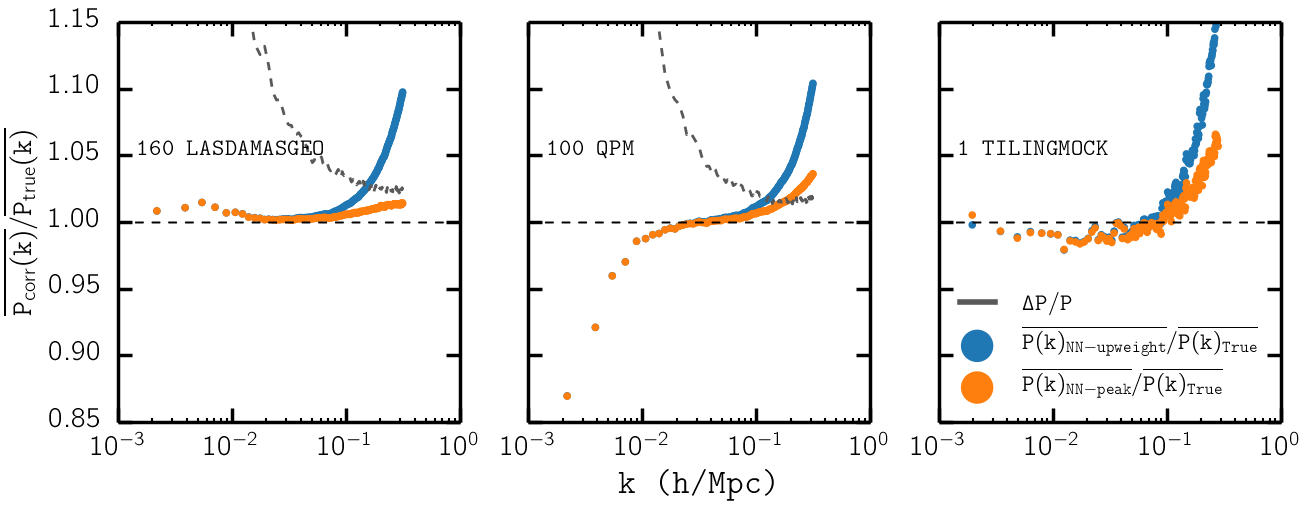
\includegraphics[scale=0.55]{fcpaper_pk_peakonly_comp.png} 
\caption{The ratio of $\overline{P_\mathrm{corr} (k)}$ using the nearest-neighbor (NN) correction (blue) and $d_\mathrm{LOS}$-peak correction (orange) over the true $\overline{P(k)}$ for LasDamas (left panel), QPM (middle panel), and Tiling Mock (right panel) catalogs. The NN correction and $d_\mathrm{LOS}$-peak correction methods are described in Section \ref{sec:dlos}. We also plot the ratio of the sample variance to the true $\overline{P_\mathrm{truee}(k)}$, $\Delta P_\mathrm{true}(k) / \overline{P_\mathrm{true}(k)}$ (black; dashed) for comparison. Incorporating the $d_{\mathrm{LOS}}$ distribution significantly improves the correction of fiber collisions for $k > 0.1 \; h/\mathrm{Mpc}$; however, neither method is able to constrain the systematic effects of fiber collisions significantly below the sample variance at $k > 0.2 \; h/\mathrm{Mpc}$.}\label{fig:peakonly}
\end{center}
\end{figure*}

The $d_\mathrm{LOS}$-peak correction is the first part of our correction method we present in this paper. We test it by applying it to the mock catalogs and comparing the resulting power spectrums. For each of the mock catalogs (LasDamas, QPM, and Tiling Mock) we use the FKP power spectrum estimator from Section \ref{sec:pk_est} to compute the power spectrums of the mock catalogs without fiber collisions, with fiber collisions corrected using NN method, and with fiber collisions corrected using the $d_\mathrm{LOS}$-peak correction. We note that both the NN and the $d_\mathrm{LOS}$-peak correction methods alter the redshift distribution of our samples by a negligible amount $< 1\%$. Therefore, the synthetic random catalogs and the $\bar{n}(z)$ values do not need to be adjusted in the FKP $P(k)$ calculations in our case. 

Since we are interested in how well fiber collision correction methods can reproduce the power spectrum without fiber collisions (i.e. ``true" power spectrum, unsullied by systematic effects), in Figure \ref{fig:peakonly} we plot the ratio of the average power spectrum $\overline{P(k)}$ (averaged over the realizations) computed from fiber collided mock catalogs with corrections over the $\overline{P(k)}$ from the fiber collision-less original mock catalogs: $\overline{P_{\mathrm{corr}}(k)}/\overline{P_\mathrm{true}(k)}$. The ratio for the NN method is plotted in blue while the ratio for the $d_{\mathrm{LOS}}$-peak correction is plotted in orange. We also plot $\Delta P_\mathrm{true}(k) / \overline{P_\mathrm{true}(k)}$ (black; dashed) in order to compare the ratios to sample variance of the mock catalogs. $\Delta P_\mathrm{true}(k)$ is computed using Eq. \ref{eq:pk_var}. At large scales ($k < 0.1 \; h/\mathrm{Mpc}$), for all mock catalogs, both fiber collision methods are able to reasonably reconstruct the true power spectrum. At small scales on the other hand, the $\overline{P_\mathrm{NN}(k)}$ is greater than $\overline{P_\mathrm{true}(k)}$ by $> 10 \%$ at $ k \sim 0.3\; h/\mathrm{Mpc}$. In comparison, the $d_\mathrm{LOS}$-peak method significantly improves this residual to $\sim 5\%$ greater than $P_\mathrm{true}(k)$ at $k \sim 0.3 \; h/\mathrm{Mpc}$. {\bf include more description of even smaller scales when the figures are ready}. 

When we compare the NN method and the $d_\mathrm{LOS}$-peak correction to the sample variance ratio ($\Delta P_\mathrm{true}(k) / \overline{P_\mathrm{true}(k)}$), we find that neither of these methods sufficiently correct for fiber collisions at $k > 0.1\; h/\mathrm{Mpc}$. The $P(k)$s obtained from these methods are dominated by the systematic effects of fiber collisions on small scales. Although the $d_\mathrm{LOS}$-peak method improves upon the NN method by statistical reconstructing the clustering of correlated fiber collided pairs within the peak of the $d_\mathrm{LOS}$ distribution, there is still room for improvement since the method does not yet properly account for chance alignments (uncorrelated fiber collision pairs). Unfortunately, an extension of the $d_\mathrm{LOS}$-peak method to the entire $d_\mathrm{LOS}$ distribution range is not feasible because such a correction results in an overall reduction of the $P(k)$. This is caused by the statistical sampling of the $d_\mathrm{LOS}$, which would inevitably displace some fiber collided pairs that are actually correlated pairs as chance alignments and the other way around. Therefore, in the following section we provide more robust correction method to account for the chance alignment fiber collided pairs. 

\begin{figure*}
\begin{center}
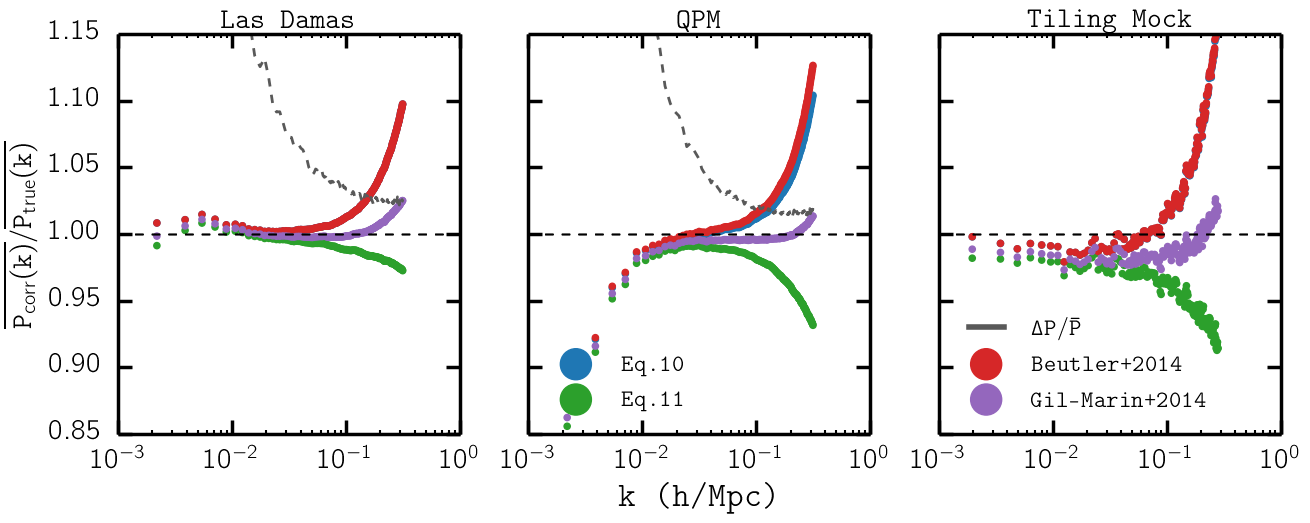
\includegraphics[scale=0.55]{fcpaper_pk_shotnoiseonly_comp.png}
\caption{The ratio of $\overline{P_\mathrm{SN}(k)}$ computed using the shot-noise correction term given by Eq. \ref{eq:fkp_shotnoise} (blue), Eq. \ref{eq:ourshot} (green), $P^\mathrm{B2014}_\mathrm{shot}$ (red), and $P^{\mathrm{GM2014}}_\mathrm{shot}$ (purple) over $\overline{P_\mathrm{true}(k)}$ for LasDamas (left panel), QPM (middle panel), and Tiling Mock (right panel) catalogs. We also plot $\Delta P_\mathrm{true}/P_\mathrm{true}(k)$ to compare with the sample variance ratio. $\overline{P_\mathrm{SN}(k)}$ computed using Eq. \ref{eq:fkp_shotnoise} shot-noise correction is identical to the NN method $\overline{P_\mathrm{corr}(k)}$ presented in Figure \ref{fig:peakonly} and as before significantly overestimates $\overline{P_\mathrm{true}(k)}$ at $k > 0.1 \; h/\mathrm{Mpc}$. $\overline{P_\mathrm{SN}(k)}$ using $P^\mathrm{B2014}_\mathrm{shot}$ equivalently overestimates $\overline{P_\mathrm{true}(k)}$ at $k > 0.1 \; h/\mathrm{Mpc}$. On the other hand $\overline{P_\mathrm{SN}(k)}$ computed using Eq. \ref{eq:ourshot} significantly underestimates the power spectrum at $k > 0.1 \; h/\mathrm{Mpc}$ with $\overline{P^\mathrm{Eq.15}_\mathrm{SN}}/\overline{P_\mathrm{true}}(k \sim 0.3) -1 \sim -3 \%, -8 \%, \;\mathrm{and} -9$ for LasDamas, QPM, and Tiling Mock respectively. $\overline{P_\mathrm{SN}(k)}$ computed using $P^\mathrm{GM2014}_\mathrm{shot}$ provides the best correction for fiber collisions ($\overline{P^\mathrm{GM2014}_\mathrm{SN}}/\overline{P_\mathrm{true}}(k \sim 0.3) -1 \sim 2.5 \%$). However at these small scales, even for $\overline{P^\mathrm{GM2014}_\mathrm{SN}}$ the effect of fiber collisions is comparable to sample variance at $k \sim 0.3 \;h/\mathrm{Mpc}$. } \label{fig:shotnoise}
\end{center}
\end{figure*}
%%%%%%%%%%%%%%%%%%%%%%%%%%%%%%%%%%%%%%%%%%%%%%%%%%%%%%%%%%%%%%%%%%%%%%%%%%%%%%
% SHOT NOISE CORRECTION 
%%%%%%%%%%%%%%%%%%%%%%%%%%%%%%%%%%%%%%%%%%%%%%%%%%%%%%%%%%%%%%%%%%%%%%%%%%%%%%
\subsection{Shot Noise Correction} \label{sec:shotnoise} 
Both the NN method and the $d_\mathrm{LOS}$-peak correction do not sufficiently account for the systematic effects of fiber collisions in the power spectrum. In this section we introduce the other part of our fiber collision correction method that involve the shot-noise correction term of the FKP power spectrum estimator. By modifying the shot noise term of the FKP estimator to account for fiber collisions, we present a more robust correction method that accounts for the chance aligned fiber collided pairs. 

In Section \ref{sec:catalog}, we described the FKP power spectrum estimator used to compute the power spectrums of Figure \ref{fig:mockpk}. In their estimator, to account for the discreteness of the density field, they subtract the shot-noise contribution to the power spectrum (Equation \ref{eq:fkppk}): 
\begin{equation} \label{eq:fkp_sn_int}
P_\mathrm{shot} = \frac{ (1+\alpha) \int d^3r \;\bar{n}({\bf r})w^2({\bf r})}{\int d^3r \;\bar{n}^2({\bf r})w^2({\bf r})}. 
\end{equation}
In practice, the integrals in Equation \ref{eq:fkp_sn_int} can be written in terms of discrete sums over the random catalog. The spatial integral $\int d^3r \; \bar{n}({\bf r}) ...$ can be computed as the discrete sum $\alpha \sum_{\mathrm{ran}}...$. With this conversion,
\begin{equation} \label{eq:fkp_shotnoise}
P^\mathrm{FKP}_\mathrm{shot} = \frac{(1+\alpha) \alpha \sum\limits_{\mathrm{random}} w_\mathrm{FKP}^2({\bf r})}{\alpha \sum\limits_{\mathrm{random}}w_\mathrm{FKP}^2({\bf r})}.
\end{equation} 
However, in the FKP derivation, they do not take systematic weights of galaxies into account.

The spatial integral $\int d^3r \;\bar{n}({\bf r})...$ can also be computed using the mock catalogs rather than the synthetic random catalogs, as $\sum_{\mathrm{gal}} w_g...$ where $w_g$ represents the statistical weight assigned to the galaxies (\citealt{Cole:2005aa, Yamamoto:2006aa, Beutler:2014aa, Gil-Marin:2014aa}). Then the shot-noise component can be expressed as: 
\begin{equation} \label{eq:fkpweight}
P_\mathrm{shot} = \frac{ \sum\limits_{\mathrm{galaxy}} w^2_\mathrm{FKP}w^2_g({\bf r})- \alpha^2 \sum\limits_{\mathrm{random}} w_\mathrm{FKP}^2({\bf r})}{\alpha \sum\limits_{\mathrm{random}}w_\mathrm{FKP}^2({\bf r})}.
\end{equation}
In this form, systematic weights for galaxies can be accounted for in the $w_g$ and $\alpha$ terms. 

Following the latter formulation, most recently, both \cite{Beutler:2014aa} and \cite{Gil-Marin:2014aa} formulate $P_\mathrm{shot}$ to account for systematic bias in their analysis of BOSS data. However, systematic weights are treated differently in each of their derivation. Keeping in mind the weights listed in Eq. \ref{eq:weight} for the BOSS data, \cite{Beutler:2014aa} derives
\begin{equation} \label{eq:florian}
P^\mathrm{B2014}_\mathrm{shot} = \frac{\sum\limits_{\mathrm{galaxy}} w^2_\mathrm{FKP}w_\mathrm{tot}({\bf r})w_\mathrm{sys}({\bf r}) - \alpha'^2 \sum\limits_{\mathrm{random}} w_\mathrm{FKP}^2({\bf r})}{\alpha' \sum\limits_{\mathrm{random}}w_\mathrm{FKP}^2({\bf r})}, 
\end{equation}
where $\alpha' = \sum_\mathrm{gal} w_\mathrm{tot} / N_\mathrm{ran}$. 

On the other hand, \cite{Gil-Marin:2014aa}, in a formulation designed to account for fiber collisions derives $P_\mathrm{shot}$ using two separate components: one for correlated pairs and the other chance alignments. The shot-noise contribution to the power from correlated pairs (referred to as ``true pairs" in \citealt{Gil-Marin:2014aa}) is equivalent to Eq. \ref{eq:florian} above ($P_\mathrm{shot}$ in \cite{Beutler:2014aa}). For chance alignments (referred to as ``false pairs" in \citealt{Gil-Marin:2014aa}), the shot-noise contribution is derived as, 
\begin{equation} \label{eq:gm_falsepairs}
P^\mathrm{False}_\mathrm{shot} = \frac{\sum\limits_{\mathrm{galaxy}} w^2_\mathrm{FKP}w^2_\mathrm{tot}({\bf r}) - \alpha'^2 \sum\limits_{\mathrm{random}} w_\mathrm{FKP}^2({\bf r})}{\alpha' \sum\limits_{\mathrm{random}}w_\mathrm{FKP}^2({\bf r})}.
\end{equation}
Then the total $P_\mathrm{shot}$ is calculated as a combination of $P^\mathrm{True}_\mathrm{shot}$ and $P^\mathrm{False}_\mathrm{shot}$: 
\begin{equation} \label{eq:gm_shot}
P^\mathrm{GM2014}_\mathrm{shot} = (1- x_\mathrm{PS}) P^{True}_\mathrm{shot} + x_\mathrm{PS} P^{False}_\mathrm{shot}
\end{equation}
For analyzing BOSS $P(k)$ \cite{Gil-Marin:2014aa} uses $x_\mathrm{PS} = 0.58$. The $x_\mathrm{PS}$ is calculated from the weighted galaxy catalog of \cite{Manera:2013aa}, not the observed BOSS data, and it is the value that optimizes the fit of the fiber collision corrected $P(k)$ to the $P_\mathrm{true}(k)$ .  

In our $P(k)$ calculations we use the FKP estimator with the shot-noise correction term computed as Eq. \ref{eq:fkpweight} with $w_\mathrm{g} = w_\mathrm{tot}$, which gives us, 
\begin{equation} \label{eq:ourshot}
P^\mathrm{Hahn+}_\mathrm{shot} = \frac{\sum\limits_{\mathrm{galaxy}} w^2_\mathrm{FKP}w^2_\mathrm{tot}({\bf r}) - \alpha'^2 \sum\limits_{\mathrm{random}} w_\mathrm{FKP}^2({\bf r})}{\alpha' \sum\limits_{\mathrm{random}}w_\mathrm{FKP}^2({\bf r})}.
\end{equation}
We note that the difference between Eq. \ref{eq:ourshot} and Eq. \ref{eq:florian} lies in the first term of the numerator. In this term, for Eq. \ref{eq:florian}, $w_\mathrm{fc}$ is only included in $w_\mathrm{tot}$ and not in the $w_\mathrm{sys}$ term. However, Eq. \ref{eq:ourshot} accounts for fiber collisions in the $w_\mathrm{tot}^2$ term. Also, Eq. \ref{eq:ourshot} is equivalent to the shot-noise contribution from ``false pairs" in \cite{Gil-Marin:2014aa}. 
%In \cite{Gil-Marin:2014aa}, they justify the use of the two separate shot-noise terms with the argument that, if the fiber collided pairs are true pairs it would not modify %insert reason 
%While the $P(k)$ using the \cite{Gil-Marin:2014aa} shot-noise term does in fact correct for fiber collisions significantly (below), since the parameter is determined in mock catalogs, the value cannot be validated in the actual BOSS data .

In order to compare the different $P_\mathrm{shot}$ derivations, we apply each of them ($P^\mathrm{FKP}_\mathrm{shot}$, $P^\mathrm{Hahn+}_\mathrm{shot}$, $P^\mathrm{B2014}_\mathrm{shot}$ and $P^\mathrm{GM2014}_\mathrm{shot}$) to the fiber collided mock catalogs with nearest-neighbor weights. To clarify, $P^\mathrm{FKP}_\mathrm{shot}$, $P^\mathrm{Hahn+}_\mathrm{shot}$, $P^\mathrm{B2014}_\mathrm{shot}$ and $P^\mathrm{GM2014}_\mathrm{shot}$ are calculated using Eq. \ref{eq:fkp_shotnoise}, \ref{eq:ourshot}, \ref{eq:florian} and \ref{eq:gm_shot}, respectively. In our considerations of systematic effects beside fiber collisions in Eq. \ref{eq:weight}, we note that only the QPM mock catalog assigns $w_\mathrm{sys}$ (systematic weights due to sector completeness) to its galaxies and none of the mock catalogs assign $w_\mathrm{rf}$ to their galaxies. Therefore in Equations 9 - 15, for LasDamas and Tiling mock catalogs we use $w_\mathrm{sys} = w_\mathrm{rf} = 1$ so $w_\mathrm{tot} = w_\mathrm{fc}$ and for QPM mocks, we use $w_\mathrm{tot} = w_\mathrm{sys} w_\mathrm{fc}$. We compute the $P_\mathrm{SN}(k)$s using the FKP estimator with different $P_\mathrm{shot}$ prescriptions for each of the mock catalogs. We then average the power spectrum over the realizations to get $\overline{P_\mathrm{SN}(k)}$s for the mock catalogs, and then take the ratio over $\overline{P_\mathrm{true}(k)}$. 

In Figure \ref{fig:shotnoise}, we present $\overline{P_\mathrm{SN}(k)}/\overline{P_\mathrm{true}(k)}$ computed using $P^\mathrm{FKP}_\mathrm{shot}$, $P^\mathrm{Eq.\ref{eq:ourshot}}_\mathrm{shot}$, $P^\mathrm{B2014}_\mathrm{shot}$ and $P^\mathrm{GM2014}_\mathrm{shot}$ shot noise correction term equations. $\overline{P_\mathrm{SN}(k)}$ calculated using $P^\mathrm{FKP}_\mathrm{shot}$ is the identical to the NN corrected $\overline{P(k)}$ in Figure \ref{fig:peakonly}. Hence as before, it over estimates the $\overline{P_\mathrm{true}(k)}$ by $> 10 \%$ for all mocks at $k \sim 0.3 \; h/\mathrm{Mpc}$. $\overline{P(k)}$ measured using $P^\mathrm{B2014}_\mathrm{shot}$ (Eq. \ref{eq:florian}) does not significantly improve this overestimation in any of the mock catalogs. In fact for LasDamas and Tiling mock catalogs, since $w_\mathrm{sys} = 1$, $P^\mathrm{FKP}_\mathrm{shot} = P^\mathrm{B2014}_\mathrm{shot}$. Even for QPM, which assigns $w_\mathrm{sys}$ to its galaxies there are no significant improvements from using $P^\mathrm{B2014}_\mathrm{shot}$ over $P^\mathrm{FKP}_\mathrm{shot}$. 

On the other hand, $\overline{P(k)}$ using Eq. \ref{eq:ourshot} significantly is significantly lower than the $\overline{P_\mathrm{true}(k)}$. $\overline{P^\mathrm{Eq.\ref{eq:ourshot}}_\mathrm{SN}}/\overline{P_\mathrm{true}}(k\sim0.3) - 1 \sim -3 \%, -8 \%, \;\mathrm{and} -9$ for LasDamas, QPM, and Tiling Mock respectively. Finally, $\overline{P(k)}$ measured using $P^\mathrm{GM2014}_\mathrm{shot}$ reproduces $\overline{P_\mathrm{true}(k)}$ most accurately in the comparison of Figure \ref{fig:shotnoise}. $\overline{P^\mathrm{GM2014}_\mathrm{SN}}/\overline{P_\mathrm{true}}(k\sim 0.3) -1 \sim 2.5 \%$. As in Figure \ref{fig:peakonly}, we again plot the sample variance ($\Delta P/\bar{P}$) for each of the mock catalogs in Figure \ref{fig:shotnoise} for comparison. $\overline{P(k)}$ computed using $P^\mathrm{Gil-Marin}_\mathrm{shot}$ is able to best constrain the effects of fiber collisions in our comparison. However, even $\overline{P^\mathrm{GM2014}_\mathrm{SN}}$ is unable to significantly reduce the effects of fiber collisions below the sample variance, especially near $k \sim 0.3 \;h/\mathrm{Mpc}$. 

The shot-noise correction term we present in Eq. \ref{eq:ourshot} should only correct for the shot-noise contribution to the power spectrum from chance alignment fiber collided pairs - not from correlated pairs. Because we apply the shot-noise correction to all fiber collided pairs indiscriminately in Figure \ref{fig:shotnoise}, the shot-noise correction term over-subtracts the power spectrum as we find in Figure \ref{fig:shotnoise}. In the following section we present our fiber collision correction method, that combines the $d_\mathrm{LOS}$-peak correction of Section \ref{sec:dlos} and Eq. \ref{eq:ourshot} from this section. 


\begin{figure*}
\begin{center}
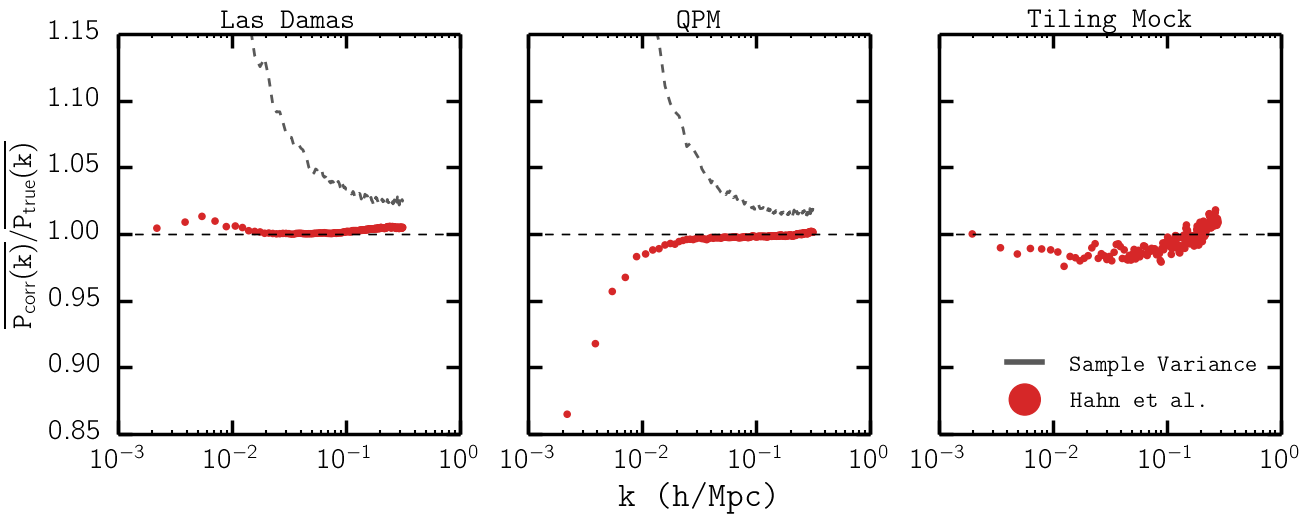
\includegraphics[scale=0.55]{fcpaper_pk_peakshotnoise_mpfit_comp.png} 
\caption{The ratio of $\overline{P(k)}$ computed using our fiber collision correction method presented in Section \ref{sec:apply} over $\overline{P_\mathrm{true}(k)}$ for LasDamas (left panel), QPM (middle panel), and Tiling Mock (right panel) catalogs with nearest-neighbor fiber collision weights (red). We again plot $\Delta P_\mathrm{true}/P_\mathrm{true}(k)$ for comparison. $\overline{P_\mathrm{corr}}/\overline{P_\mathrm{true}}(k \sim 0.3 \; h/\mathrm{Mpc})-1 \sim 0.5\%$ for our fiber collision correction. This is significantly better than the correction methods of \cite{Anderson:2012aa}, \cite{Beutler:2014aa} and \cite{Gil-Marin:2014aa} in Figure \ref{fig:shotnoise}. Moreover, for LasDamas and QPM, our correction method is able to correct for the effects of fiber collisions, significantly below the $\Delta P_\mathrm{true}/P_\mathrm{true}(k)$ throughout the probed $k$ range, even at the smallest scales. }\label{fig:peaksn}
\end{center}
\end{figure*}
%%%%%%%%%%%%%%%%%%%%%%%%%%%%%%%%%%%%%%%%%%%%%%%%%%%%%%%%%%%%%%%%%%%%%%%%%%%%%%%%
% RESULT
%%%%%%%%%%%%%%%%%%%%%%%%%%%%%%%%%%%%%%%%%%%%%%%%%%%%%%%%%%%%%%%%%%%%%%%%%%%%%%%%
\section{Results} \label{sec:results}
\subsection{fiber collision Correction Method} \label{sec:apply}
In Section \ref{sec:dlos} we derive a method to better statistically reconstruct the clustering of correlated fiber collided pairs using using the peak of the $d_\mathrm{LOS}$ distribution. Then in Section \ref{sec:shotnoise} we presented our formulation of the shot-noise correction term, which accounts for the added discreteness from chance aligned fiber collision pairs. We now combine these two methods and present our fiber collision correction method. 

We begin once again with the fiber collided mock catalogs with the nearest-neighbor weights that accurately imitate the effects of fiber collision on the actual observed BOSS data. Then as described in Section \ref{sec:dlos}, we calculate the $d_\mathrm{LOS}$ distribution of all fiber collided pairs in each mock catalog. From the $d_\mathrm{LOS}$ distribution, we compute the fraction of fiber collided pairs within the peak of the distribution ($f_\mathrm{peak}$; Section \ref{sec:dlos}). We then select $f_\mathrm{peak}$ of the fiber collided pairs and designate them as correlated pairs that lie within the peak of the $d_\mathrm{LOS}$ distribution. We refer to these fiber collided pairs as ``peak-assigned" pairs.  

Each of these ``peak-assigned" pairs, by the nearest-neighbor weights, consist of a galaxy with $w_\mathrm{fc} > 1$ (the ``nearest-neighbor" galaxy) and another with $w_\mathrm{fc} = 0$ (the ``collided" galaxy). We disregard the collided galaxy. For each of the nearest-neighbor galaxies, we sample a value $d_\mathrm{peak-assigned}$ from the Gaussian best-fit to the $d_\mathrm{LOS}$ distribution peak and place a galaxy with $w_\mathrm{fc} = 1$ at a comoving distance $d_\mathrm{peak-assigned}$ away from the nearest-neighbor galaxy. At the same time, we reduce $w_\mathrm{fc}$ of the nearest-neighbor galaxy (the one that was originally up-weighted) by $1$. This process is repeated until the nearest-neighbor galaxy has $w_\mathrm{fc} =1$ in the case of triplets or higher. 

We keep the nearest-neighbor fiber collision weights imposed in the beginning for the remaining fiber collided pairs that are not ``peak-assigned" ($1-f_\mathrm{peak}$ of the fiber collided pairs). The resulting mock catalog has $f_\mathrm{peak}$ fewer galaxies with $w_\mathrm{cp} > 1$ compared to the fiber collided mock catalogs with nearest-neighbor weights that we started from; however, the total statistical weight ($\sum_\mathrm{gal} w_\mathrm{tot}$) of the mock catalog is conserved. 

Next, we use the FKP estimator with the Eq. \ref{eq:ourshot} shot-noise correction term described in Section \ref{sec:shotnoise} to calculate the $P(k)$ for our $d_\mathrm{LOS}$-peak corrected mock catalogs. In Figure \ref{fig:peaksn}, we present the ratio of the $\overline{P(k)}$ computed using our fiber collision correction method over $\overline{P_\mathrm{true}(k)}$. To assess the merit of the fiber collision correction, we once again over-plot the sample variance of the mock catalogs. For LasDamas, at $k \sim 0.3 \; h/\mathrm{Mpc}$, $P(k)/P_\mathrm{true}(k) - 1 \sim 0.5 \%$ and throughout the $k$ range, $0.3 \% < P(k)/P_\mathrm{true}(k) - 1 < 1.3 \%$. For QPM, at $k \sim 0.3 \; h/\mathrm{Mpc}$, $P(k)/P_\mathrm{true}(k) - 1 \sim 0.04 \%$ and throughout the $k$ range, $0.3 \% < P(k)/P_\mathrm{true}(k) - 1 < 1.3 \%$. {\bf include numbers here when Ngrid=960 is done}. Moreover for the mock catalogs with sample variance measurements (LasDamas and QPM), the $P(k)$ ratio is significantly below the sample variance throughout the entire $k$ range probed and even at $k\sim 0.3\;h/\mathrm{Mpc}$. 

%%%%%%%%%%%%%%%%%%%%%%%%%%%%%%%%%%%%%%%%%%%%%%%%%%%%%%%%%%%%%%%%%%%%%%%%%%%%%%%%
% Goodness of fit
%%%%%%%%%%%%%%%%%%%%%%%%%%%%%%%%%%%%%%%%%%%%%%%%%%%%%%%%%%%%%%%%%%%%%%%%%%%%%%%%
\subsection{Goodness-of-fit} \label{sec:litcomp}
%%%%%%%%%%%%%%%%%%%%%%%%%%%%%%%%%%%%%%%%%%%%%%%% CHI-SQUARED FIGURE 
\begin{figure*} 
\begin{center}
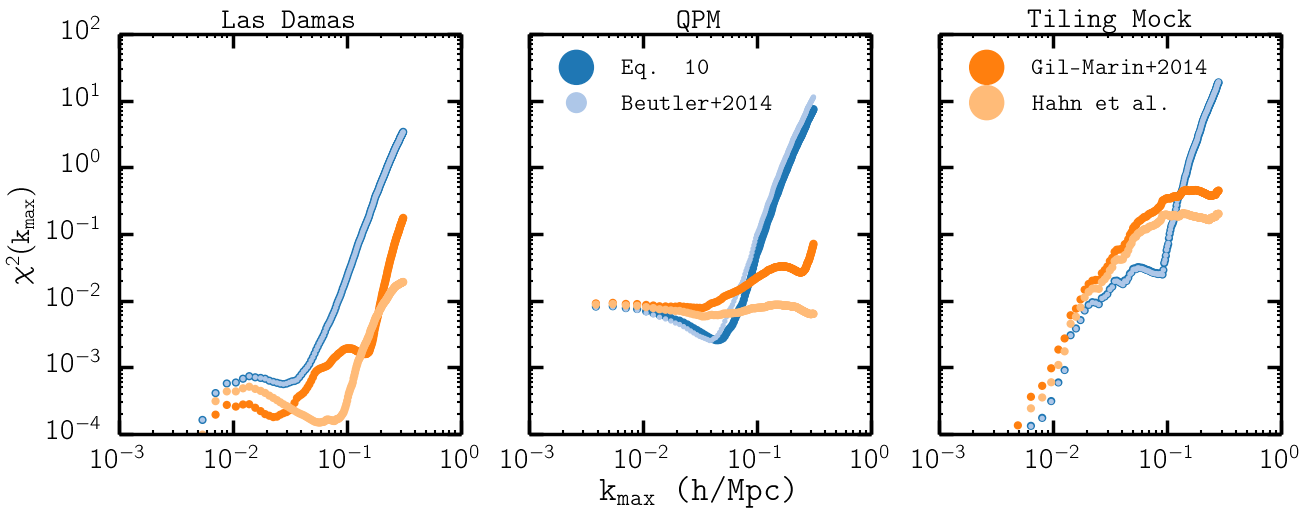
\includegraphics[scale=0.55]{fcpaper_pk_chisquared_comparison.png} 
\caption{$\chi^2 (k_\mathrm{max})$ for $P_\mathrm{NN-upweight}$ (blue), $P_\mathrm{Beutler}$ (light blue), $P_\mathrm{Gil-Marin}$ (orange), and $P_\mathrm{Hahn}$ (yellow) using the LasDamas (left panel), QPM (centerl panel), and Tiling (right panel) mock catalogs. Equation \ref{eq:chi2} was used to compute the $\chi^2(k_\mathrm{max})$. }\label{fig:peaksnchi2}
\end{center}
\end{figure*}
%%%%%%%%%%%%%%%%%%%%%%%%%%%%%%%%%%%%%%%%%%%%%%%% CHI-SQUARED FIGURE 

The correction method we present in this paper corrects for the effect of fiber collisions to the extent where $P_\mathrm{corr}(k)$ measurements are no longer dominated by systematic effects at the scales probed in our calculations, even for the smallest scales of $k \sim 0.3 \; h/\mathrm{Mpc}$. However, to further quantify how accurately our correction method is able to reproduce the true power spectrum and correct for the effects of fiber collisions, we quantify the goodness-of-fit for all the corrected $P(k)$s to $P_\mathrm{true}(k)$ by calculating the following $\chi^2$: 
\begin{equation}
\chi^2 (k_\mathrm{max}) = \frac{1}{N_{k_\mathrm{max}}} \sum\limits_{k< k_\mathrm{max}} \frac{(\overline{P_\mathrm{corr}(k)} - \overline{P_\mathrm{true}(k))^2}}{\Delta P_\mathrm{true} (k)^2}. \label{eq:chi2}
\end{equation}
$N_{k_\mathrm{max}}$ is the number of $k$ bins in the $P(k)$ calculation with $k < k_\mathrm{max}$. $\overline{P_\mathrm{corr}(k)}$ is the average fiber collision corrected powerspectrum of all realizations for each catalog. $\Delta P_\mathrm{true}(k)$ is the standard deviation of $P_\mathrm{true}(k)$ computed from all realizations of each mock catalog. We calculate $\chi^2$ as a function of $k_\mathrm{max}$ in order to determine the accumulated $\chi^2$ to a specific scale ($k_\mathrm{max}$). In doing so, we determine the scale to which a power spectrum analysis can be extended to without fiber collisions dominating the measurement. 

For the Tiling Mock catalog, since there is only one realization, the variance ($\Delta P_\mathrm{true} (k)$) cannot be computed independently. However, for an estimate of the $\chi^2$, we estimate $\Delta P_\mathrm{true}^\mathrm{Tiling\;Mock}(k)$ from $\Delta P^\mathrm{QPM}_\mathrm{true} (k)$ scaled by the ratio of the power spectrums:
\begin{equation}
\Delta P_\mathrm{true}^\mathrm{Tiling}(k) = \Delta P_\mathrm{true}^\mathrm{QPM}(k) \times \frac{P_\mathrm{true}^\mathrm{Tiling}(k)}{\overline{P^\mathrm{QPM}_\mathrm{true}(k)}}.
\end{equation}

In Figure \ref{fig:peaksnchi2}, we present the $\chi^2(k_\mathrm{max})$ for $P(k)$ using the following fiber collision correction methods: the NN correction (also \citealt{Anderson:2012aa}), \cite{Beutler:2014aa}, \cite{Gil-Marin:2014aa}, and our method from Section \ref{sec:apply}. The comparison is made using the LasDamas (left panel), QPM (center panel) and Tiling (right panel) mock catalogs. First in the LasDamas panel, at scales larger than $k_\mathrm{max} < 5 \times 10^{-2} \; h/\mathrm{Mpc}$, $\chi^2 < 10^{-3}$ for all correction methods, which suggests that all correction methods sufficiently correct for fiber collisions and reasonably reconstructs $P_\mathrm{true}(k)$ at these scale. In approaching smaller scales the $\chi^2$ for all correction methods increase. However, throughout the entire $k_\mathrm{max}$ range, our correction method provides a notably lower $\chi^2$ in comparison to the other correction methods. This is especially clear at $k_\mathrm{max} \sim 0.3 \; h/\mathrm{Mpc}$, where $\chi^2_\mathrm{NN} \approx 0.33$, $\chi^2_\mathrm{B2014} \approx 0.33$, and $\chi^2_\mathrm{GM2014} \approx 0.17$ while $\chi^2 \approx 0.019$ for our method. 

Next in the QPM panel (center), at scales larger than $k_\mathrm{max} < 2 \times 10^{-2} \; h/\mathrm{Mpc}$ all corrected $P(k)$ again provide a reasonable reconstruction of $P_\mathrm{true}(k)$ with $\chi^2 \approx 10^{-2}$. Then for $2 \times 10^{-2} < k_\mathrm{max} < 5 \times 10^{-2}\; h/\mathrm{Mpc}$, the NN and \cite{Beutler:2014aa} correction methods have the lower $\chi^2$s than \cite{Gil-Marin:2014aa} and our correction methods. However, as $k_\mathrm{max}$ increases, the $\chi^2$s for NN and \cite{Beutler:2014aa} quickly surpasses the $\chi^2$s of \cite{Gil-Marin:2014aa} and our method. Meanwhile, throughout the entire $k_\mathrm{max}$ range probed, our correction method has a significantly lower $\chi^2$ than the correction method of \cite{Gil-Marin:2014aa}. The difference in $\chi^2$ is again most remarkable at the smallest scales: $\chi^2 (k_\mathrm{max} \sim 0.3) \approx 7.3,\;11, \;0.068, \;\mathrm{and} \; 0.0063$ for NN, \cite{Beutler:2014aa}, \cite{Gil-Marin:2014aa} and our correction method respectively. 

Finally for the Tiling mock catalog (right panel), we find that $\chi^2(k_\mathrm{max})$ increases in a near monotonic fashion as a function of $k_\mathrm{max}$. For $k_\mathrm{max} < 4\times10^{-2} \; h/\mathrm{Mpc}$, there are no significant differences between the $\chi^2$s of any of the correction methods. Then at intermediate scales of $4\times10^{-2} < k_\mathrm{max} < 1.5\times 10^{-2} \; h/\mathrm{Mpc}$, $\chi^2$s of NN and \cite{Beutler:2014aa} are notably lower than the $\chi^2$s of \cite{Gil-Marin:2014aa} and our method. However like the other mock catalogs at smaller scales, the $\chi^2$s of NN and \cite{Beutler:2014aa} quickly increase beyond the other $\chi^2$s, ultimately both reach $\chi^2(k_\mathrm{max} \sim 0.3) \approx 13.5$. In the meantime, $\chi^2(k_\mathrm{max} \sim 0.3) \approx 0.32$ for \cite{Gil-Marin:2014aa} and $\chi^2(k_\mathrm{max} \sim 0.3) \approx 0.15$ for our correction method. Throughout the entire $k_\mathrm{max}$ our method has a lower $\chi^2$ than \cite{Gil-Marin:2014aa}. With only one realization of the Tiling mock catalog and scaled $\Delta P$, a detailed comparison of the $\chi^2$ values is difficult. Yet the $\chi^2(k_\mathrm{max})$ results for our correction provide realistic assurance that the correction method can be applied to the actually BOSS data.

Overall, regardless of catalog, for scales $k_\mathrm{max} < 3 \times 10^{-2} \;h/\mathrm{Mpc}$, the $\chi^2$ for all fiber collision corrected $P(k)$ are negligible. Then, with the exception of the LasDamas catalog, at intermediate scales of $3 \times 10^{-2} < k_\mathrm{max} < 0.15 \; h/\mathrm{Mpc}$ the NN and \cite{Beutler:2014aa} methods show the lowest $\chi^2$s. However at these intermediate scales, all of the correction methods reasonably reconstruction of the true power spectrum with $\chi^2 \ll 1$. At the smallest scales, NN and \cite{Beutler:2014aa} corrections methods no longer provide a sufficient fit to $\overline{P_\mathrm{true}(k)}$. A detailed comparison at the small scales ($k > 1.5 \times 10^{-1} \;h/\mathrm{Mpc}$) demonstrates that the fiber collision correction we present in this paper significantly better reproduces the true power spectrum than any of the other fiber collision correction methods. Furthermore, Figure \ref{fig:peaksnchi2} illustrates that throughout the entire $k_\mathrm{max}$, our correction method is able to reasonably reproduce $P_\mathrm{true}(k)$ at all scales. 
% Detailed comparison to Gil-Marin that talk about how the xps value he calculates is only validated through mock catalogs, but our method can be validated with the overlapping regions of the real data. 

\section{Summary and Discussion} \label{sec:summary}
Using simulated mock catalogs for SDSS data with realistically imposed fiber collisions, we quantify the systematic effects of fiber collisions on galaxy clustering measurements - in particular the power spectrum. Although fiber collisions have little significant effect on the power spectrum at large scales, their effect quickly overtakes the sample variance at scales smaller than $k > 0.1 \;h/\mathrm{Mpc}$. At the smallest scales that we explore in this paper, $k \sim 0.3  \;h/\mathrm{Mpc}$, fiber collisions have over a $10 \%$ effect on the power spectrum. Consequently at these small scales, measurements of the power spectrum is dominated by the uncertainties from systematic effects of fiber collisions. 

Fortunately, using the fiber collided mock catalogs used in this paper, we are able to model the distribution of the line-of-sight displacement between fiber collided pairs. With this model, we are able to statistically reconstruct the clustering fiber collided galaxies that reside in the same halo. Combining this correction with a modification of the shot-noise term in the power spectrum estimator to properly account for the discreteness added by the nearest-neighbor weights of chance aligned fiber collided pairs, we devise a new fiber collision correction method that is able to reconstruct the true power spectrum from fiber collided data even to $k \sim 0.3 \;h/\mathrm{Mpc}$. Throughout the entire $k$ range explored in our analysis, our correction method reconstructs $P_\mathrm{true}(k)$ safely within the sample variance. 

Furthermore, we compare our method to the most common nearest-neighbor correction method (\citealt{Zehavi:2002aa, Berlind:2006aa, Anderson:2012aa}) and recent correction methods presented in \cite{Beutler:2014aa} and \cite{Gil-Marin:2014aa} to demonstrate that our method most successfully reproduces the true power spectrum at small scales and most reliably at all scales for all the LasDamas, QPM, and Tiling mock catalogs. Furthermore, while the correction method of \cite{Gil-Marin:2014aa} is comparable our correction method, the parameter $x_\mathrm{PS}$ used in the method is calculated solely through a weighted galaxy mock catalog. As an added advantage, our correction method can also be callibrated by the observed data rather than only through the mock catalogs. Therefore our correction method does not depend on the accuracy of the mock catalogs, thereby making it's application to observations further reliable. 

The fiber collision correction method we present will enable us to extend our galaxy clustering analysis to smaller scales for SDSS-III BOSS and future surveys such as eBOSS or any other large fiber-fed surveys the suffer from systematic effects of fiber collisions. Our fiber collision correction method can also be extend to higher order clustering statistics such as the quadrupole of the power spectrum and the bispectrum, which we will explore in future work. 

\bigskip
We thank something something

% No need for different sections, just present the different results 
\bibliographystyle{apj}
\bibliography{fc_paper}
\end{document}